\hrulefill
\section{General rules}


Here are some general rules of good practice for your work.

\subsection{Hug the border of the object as tightly as possible}

A precise annotation like the one shown in the image~\ref{fig:goodfit} captures the entire visual element and is as close as possible to the boundaries to reduce confusion for the machine learning model.

\begin{figure}
    \centering
    \begin{subfigure}{0.48\textwidth}
        \centering
        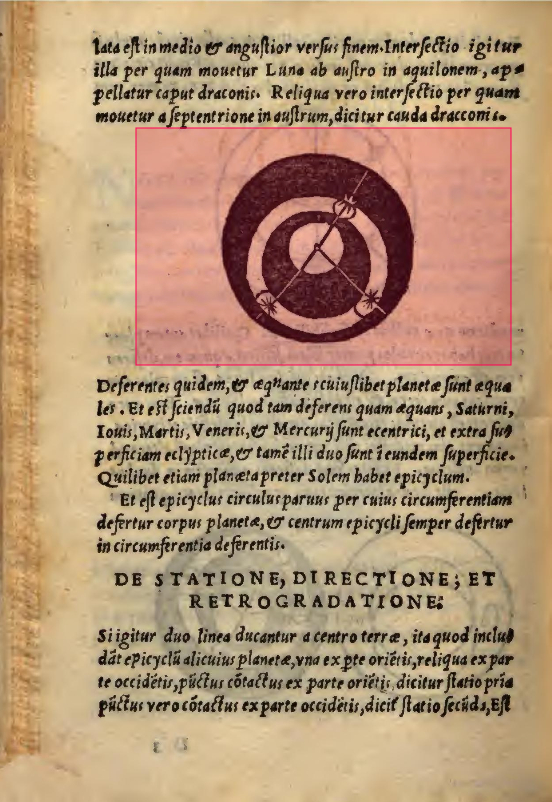
\includegraphics[width=\linewidth, height=7cm, keepaspectratio]{Guidelines/bad_fitting.png}
        \caption{ {\color{red}\faClose} Here, the annotation is too large.}
        \label{fig:badfit}
    \end{subfigure}
    \hfill
    \begin{subfigure}{0.48\textwidth}
        \centering
        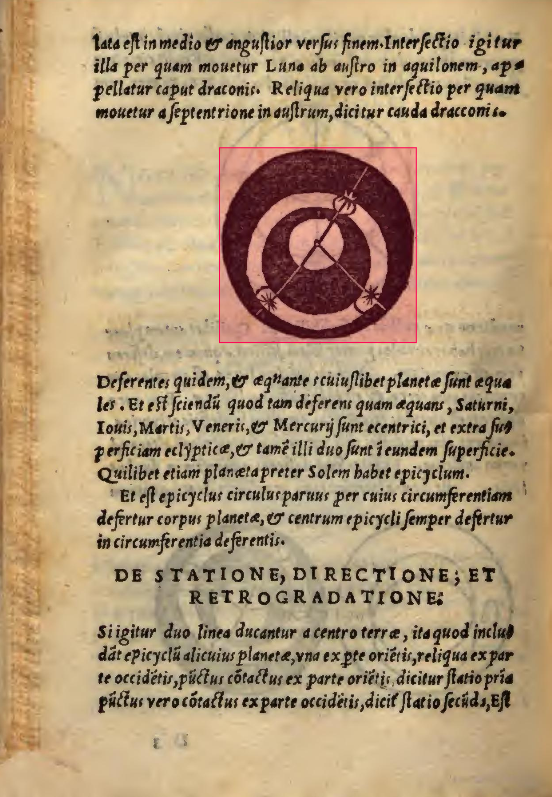
\includegraphics[width=\linewidth, height=7cm, keepaspectratio]{Guidelines/good_fitting.png}
        \caption{ {\color{green}\faCheck} Here is the correct way to annotate an element: the borders are closed to the end of the element without cutting them.}
        \label{fig:goodfit}
    \end{subfigure}
    \caption{Hug the border of the object as tightly as possible.}
\end{figure}

\subsection{Separate the elements that are not visually connected.}

Each distinct visual element must receive its own annotation (bounding box), even if several elements appear to form a coherent whole from the point of view of meaning or composition intended by the author of the document as seen in Figure~\ref{fig:unification} and Figure~\ref{fig:separation}.

Two elements can be "linked" in the author's intention (for example, a human figure and a dog figure accompanying it, or related but non-touching ornamentation) without being visually connected (that is, without sharing a common background, frame, or direct contact). In this case, the annotations are separate.

If several elements share the same background or frame (for example, several symbols or drawings printed on a single continuous graphic strip), they can be grouped into a single annotation, because they are physically or visually unified on the medium as seen in Figure~\ref{fig:example_illustration_frame} and \ref{fig:example_illustration_frame_rule} .

\begin{figure}
    \centering
    \begin{subfigure}{0.48\textwidth}
        \centering
        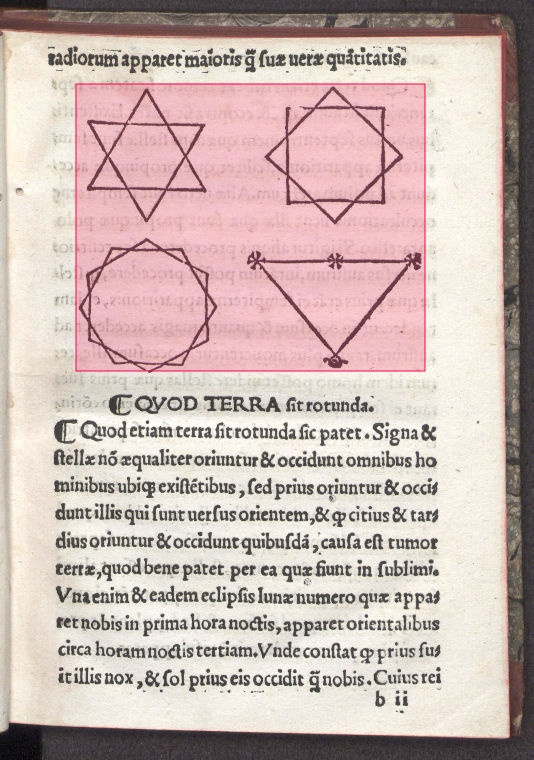
\includegraphics[width=\linewidth, height=7cm, keepaspectratio]{Guidelines/unification.png}
        \caption{{\color{red}\faClose} These elements, although clearly grouped together by the author, should not be annotated in this way.}
        \label{fig:unification}
    \end{subfigure}
    \hfill
    \begin{subfigure}{0.48\textwidth}
        \centering
        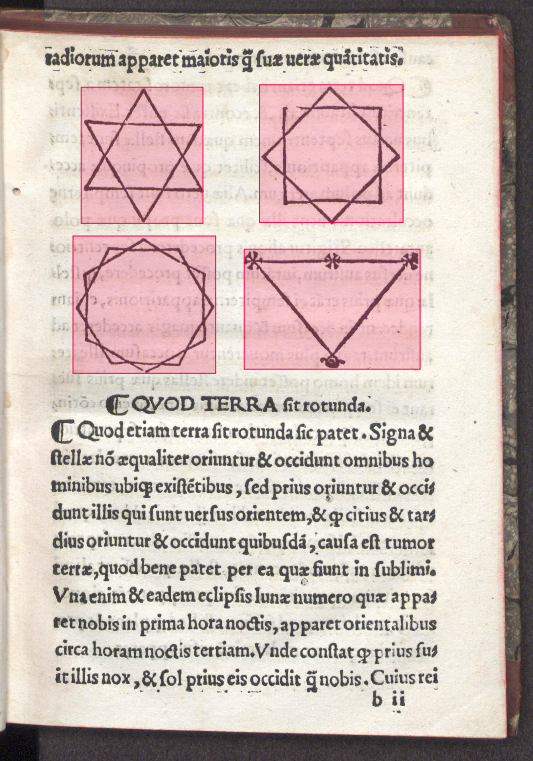
\includegraphics[width=\linewidth, height=7cm, keepaspectratio]{Guidelines/separation.png}
        \caption{{\color{green}\faCheck} Here's how we want to annotate several elements.}
        \label{fig:separation}
    \end{subfigure}
    \caption{Separate element that are not visualy linked}
\end{figure}

\subsection{Avoid item overlap} 

\textbf{This is not a strict rule}. In many documents, elements overlap and are interconnected, as illustrated in Figure \ref{fig:good_overlap}. The section on class definitions and examples will show you the cases where overlapping annotations are necessary and those where they can be avoided.

\begin{figure}
    \centering
    \begin{subfigure}{0.48\textwidth}
        \centering
        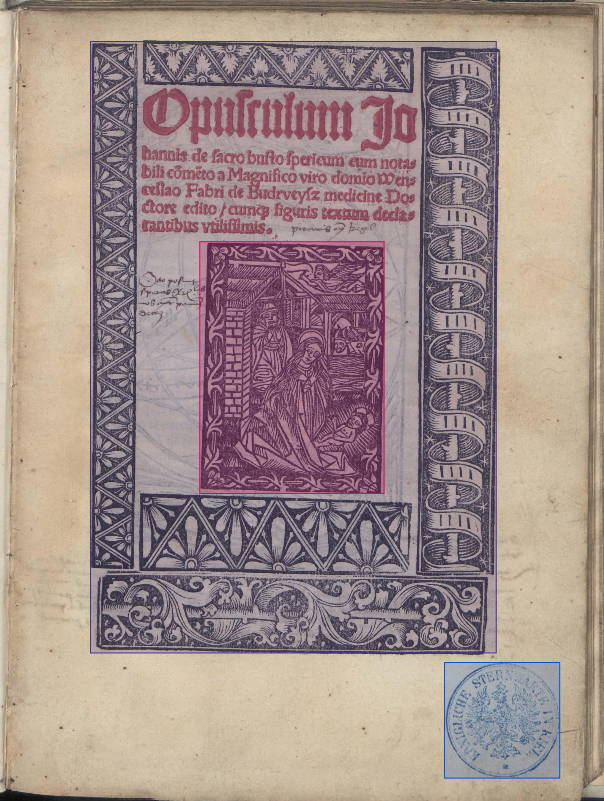
\includegraphics[width=\linewidth, height=7cm, keepaspectratio]{Guidelines/overlap.png}
        \caption{{\color{red}\faClose} The annotation of the ornament overlap against to much elements}
        \label{fig:bad_overlap}
    \end{subfigure}
    \hfill
    \begin{subfigure}{0.48\textwidth}
        \centering
        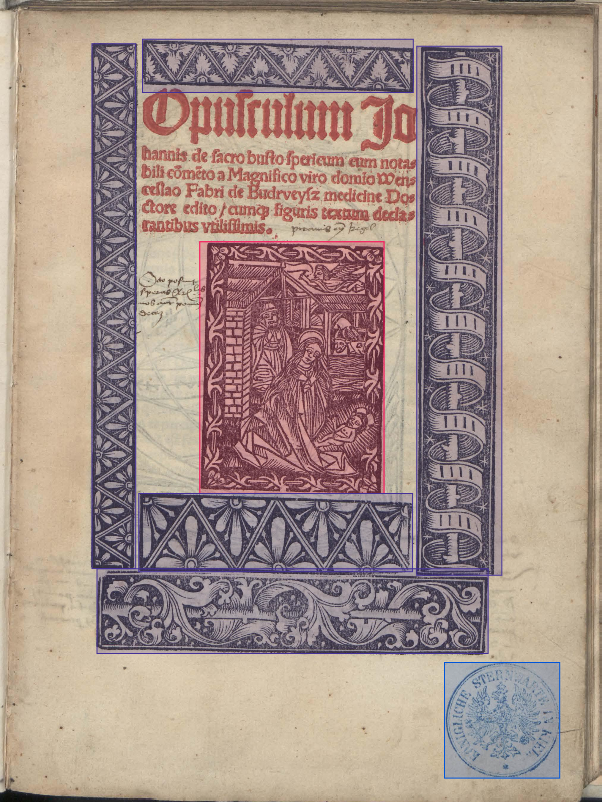
\includegraphics[width=\linewidth, height=7cm, keepaspectratio]{Guidelines/correct_overlap.png}
        \caption{{\color{green}\faCheck} We decided to cut out the decorative elements to avoid overlapping.}
        \label{fig:good_overlap}
    \end{subfigure}
    \caption{Avoid item overlap between classes}
\end{figure}

\subsection{Annotate only the main page}

Do not annotate anything that is not on the main page. As shown in example \ref{fig:main_page}, if the scan was done for two pages, annotate it as shown in \ref{fig:both_page}.

\begin{figure}
    \centering
    \begin{subfigure}{0.48\textwidth}
        \centering
        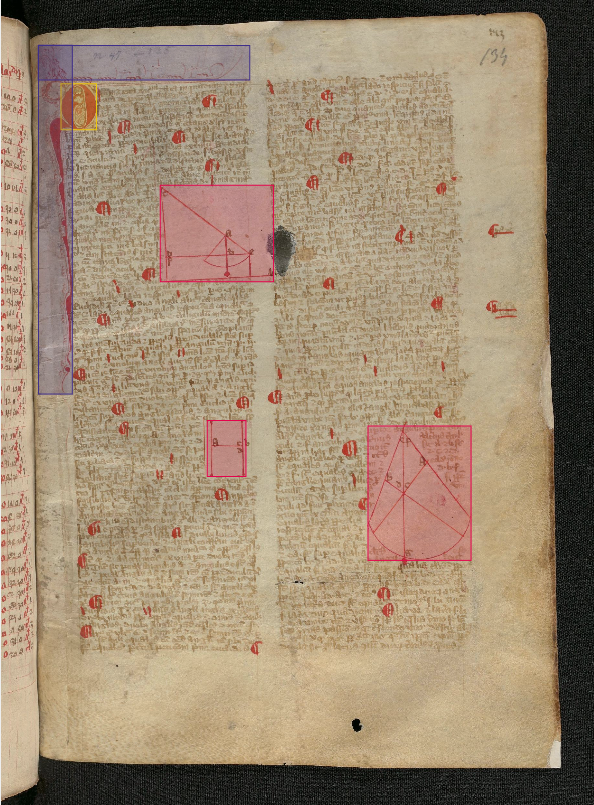
\includegraphics[width=\linewidth, height=7cm, keepaspectratio]{Guidelines/Screenshot_20260702_112821.png}
        \caption{Do not annotate the tables on the little bit of the other page.}
        \label{fig:main_page}
    \end{subfigure}
    \hfill
    \begin{subfigure}{0.48\textwidth}
        \centering
        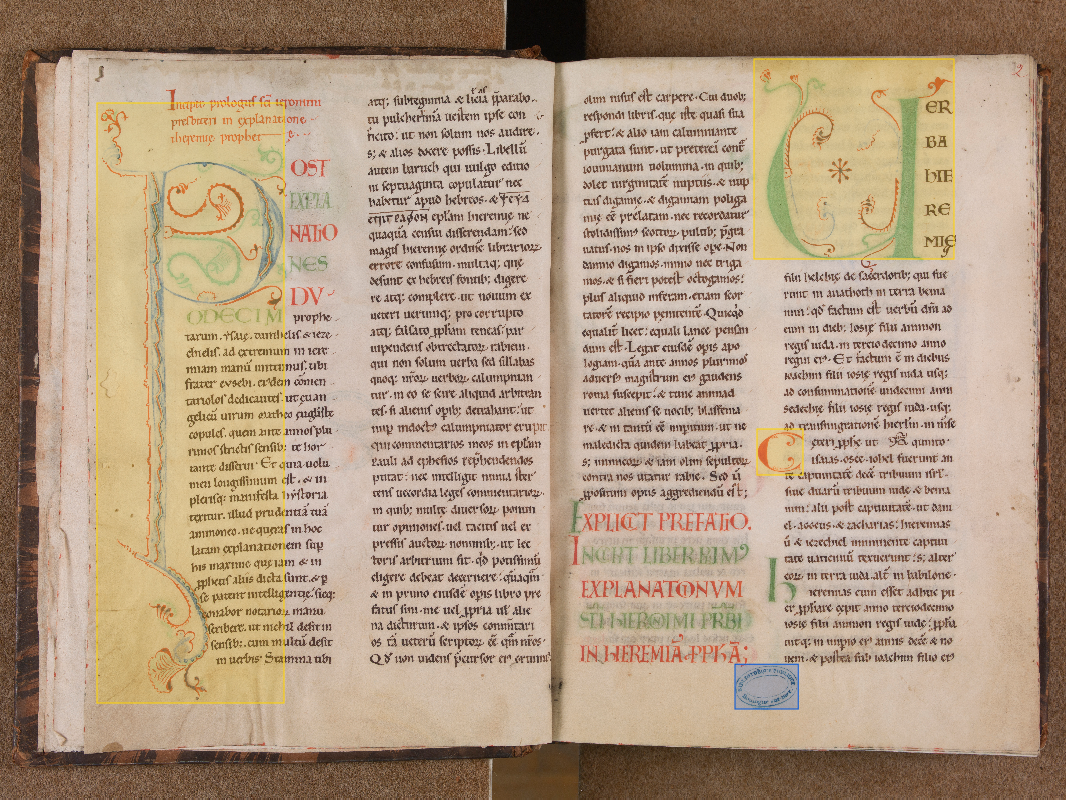
\includegraphics[width=\linewidth, height=7cm, keepaspectratio]{Guidelines/Screenshot_20260702_135302_2.png}
        \caption{If the scan is done for two pages, then you must annotate the elements of both pages.}
        \label{fig:both_page}
    \end{subfigure}
    \caption{Annotate only the main page}
\end{figure}

\subsection{Annotate what is visible, not what you infer}

Label only the content that is actually present and legible in the document, as shown in the image \ref{fig:completion}. Do not extend a bounding box or complete an area based on what you assume to be there (for example, a torn page, an erased stamp, text hidden by a fold).

\begin{figure}
    \centering
    \begin{subfigure}{0.48\textwidth}
        \centering
        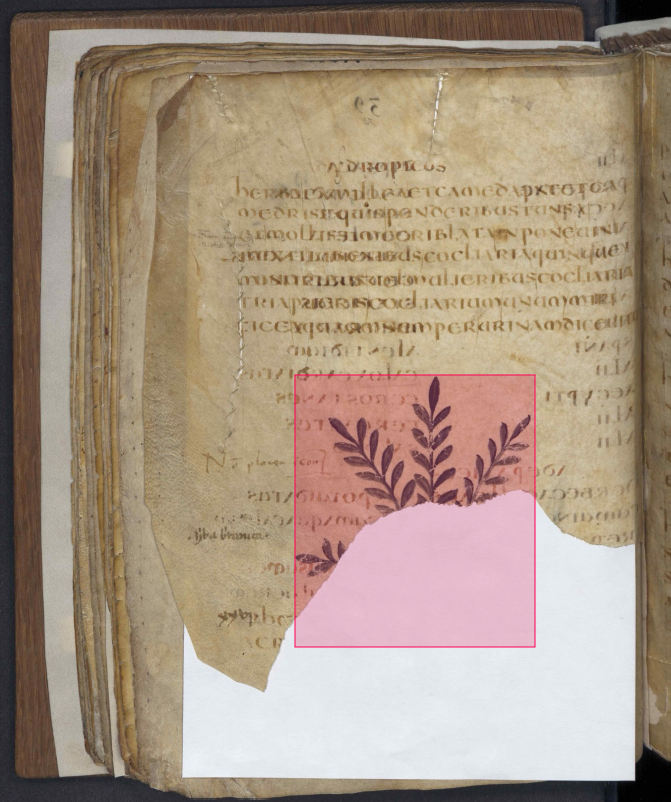
\includegraphics[width=\linewidth, height=7cm, keepaspectratio]{Guidelines/tomuch.png}
        \caption{{\color{red}\faClose} This annotation attempts to complete an element that is no longer visible.}
        \label{fig:completion}
    \end{subfigure}
    \hfill
    \begin{subfigure}{0.48\textwidth}
        \centering
        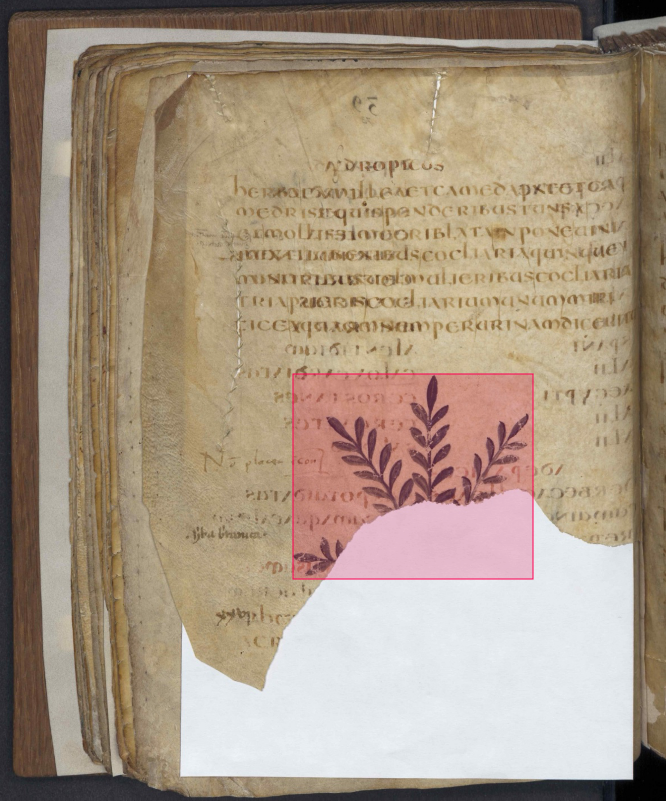
\includegraphics[width=\linewidth, height=7cm, keepaspectratio]{Guidelines/correct_amount.png}
        \caption{{\color{green}\faCheck} This annotation respects the limits of what is visible in the document.}
        \label{fig:fitting}
    \end{subfigure}
    \caption{Annotate what is visible, not what you infer}
\end{figure}

\subsection{Review your work before submitting.}

The annotation task can be arduous and tedious; it is advisable to check the quality of the annotations before moving on to the next image and to take regular breaks to stay alert and focused.